% Project: 
% Creator: 
\documentclass[11pt, letterpaper]{article}
\usepackage{text/ajps} % based on LaTex template for AJPS submission by Jeff Harden
\usepackage[authordate, backend=biber , url=false, doi=false, isbn=false]{biblatex-chicago}
\addbibresource{/Users/chaoyuewang/Desktop/Zotero.bib}

%\graphicspath{} % if graphs are stored outside the source path
%============Article Title, Authors================
 \title{\textbf{Blues in Colors: Police Violence, Racial Representation, and White Attitude Change}} 

\author{Chaoyue Wang\thanks{Chaoyue Wang (\href{mailto:chyrwang@gmail.com}{\texttt{chyrwang@gmail.com}}, 86-177-2387-5369) is a senior student of Philosophy, Politics and Economics at Yuanpei College of Peking University, Beijing, China 100871.}}
% use \and for multiple authors
%===================Startup========================
\begin{document} 
\maketitle
\onehalfspacing %\vspace{5.5in}
\thispagestyle{empty}
%===================Abstract======================= 
\begin{abstract} %    

\begin{normalsize}  \noindent   
Political behavior has been structured along group identities, and a racial division emerges regarding attitudes toward law enforcement and actions on police brutality. Compared to people of color, white Americans are more supportive of police agencies and more hesitant about reforming policing behavior even in the wake of multiple recent unjustified police-involved homicides. While existing studies attribute such difference to white's unique experiences with law enforcement, excessive white representation in police workforces has received little attention. Linking a nationally representative sample to their local context of racialized police and police violence, this study finds that more representation of black and Hispanic officers greatly enhances the process where white residents reacts to police violence by holding more critical view toward law enforcement. Interestingly, white representation in police has only weak effect of such. Findings here highlights group thinking as a contributing factor to today's racial divide on policing, and implicates how promoting racial diversity in police workforce can facilitate the outset of meaningful conversations on police violence.
\end{normalsize}
\end{abstract}

%\begin{quote}
%%\textbf{Keywords}: Keywords go here. \\
%% \noindent \textbf{Note}: Note on replication data.
%\end{quote}

%================Begin Manuscript==================
\newpage \clearpage \pagenumbering{arabic}  %\doublespacing
\setstretch{1.5}

\section{Introduction}


Political Behavior has always been structured along the boundaries of social and political identities \parencite{eganIdentityDependentVariable2020, masonUncivilAgreementHow2018, kaneWhoPartyGroup2021, jeffersonSeeingBlueBlack2021}. 
\section{Race and Police}


\section{Empirical Strategy}
\section{Results}
\section{Conclusion and Discussion}

%===================References=====================
%\newpage
%\bibliographystyle{text/chicago-apsr}
\printbibliography
%===================Appendix=====================
\newpage
\begin{appendix}
\counterwithin{figure}{section}
\counterwithin{table}{section}

\section{Graphs in Waiting}
\begin{figure}[t]
    \centering
    \caption{Distribution of Racial Imagery of Police Departments Surveyed in LEMAS 2016} 
	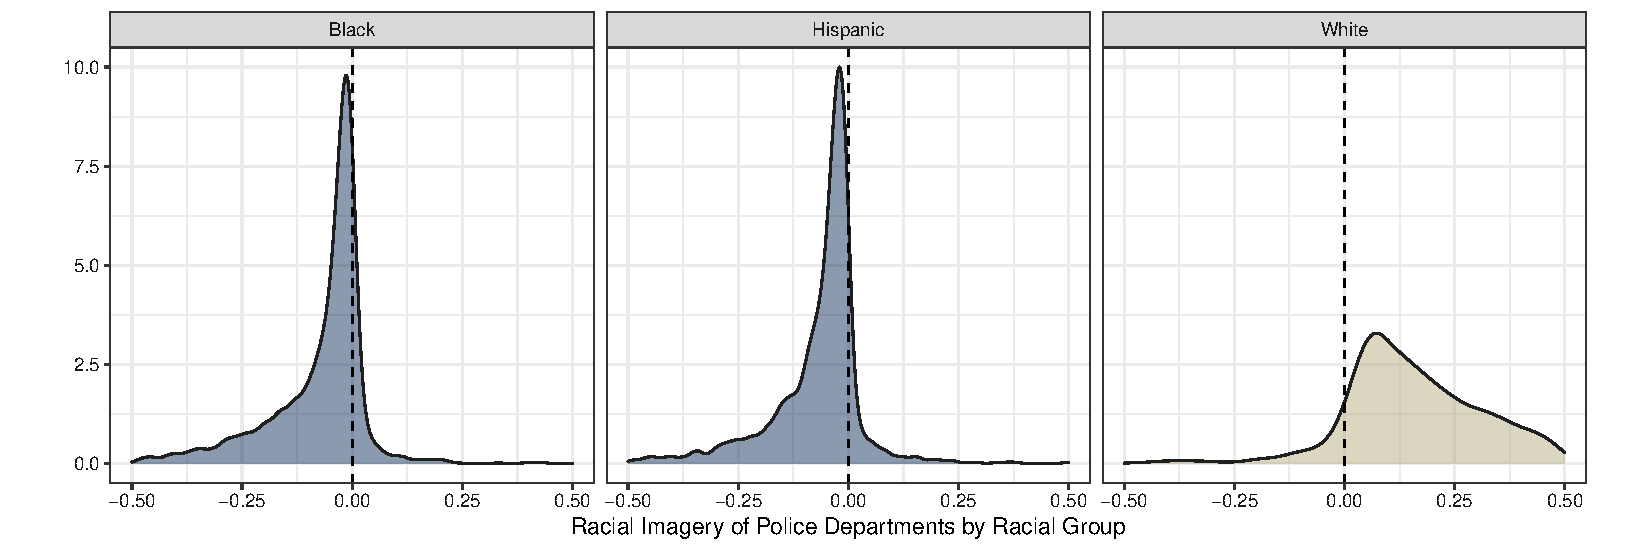
\includegraphics[width = \linewidth]{figures/desc-lemas2.pdf}
    \label{fig:lemas-density}
    \fnote{On the horizontal axis, a positive value indicates that the corresponding racial group is excessively represented in local police departments, and a negative value the otherwise.}
\end{figure}

\begin{figure}[t]  \centering
    \caption{Geographic Coverage of LEMAS 2016 at the County Level} 
	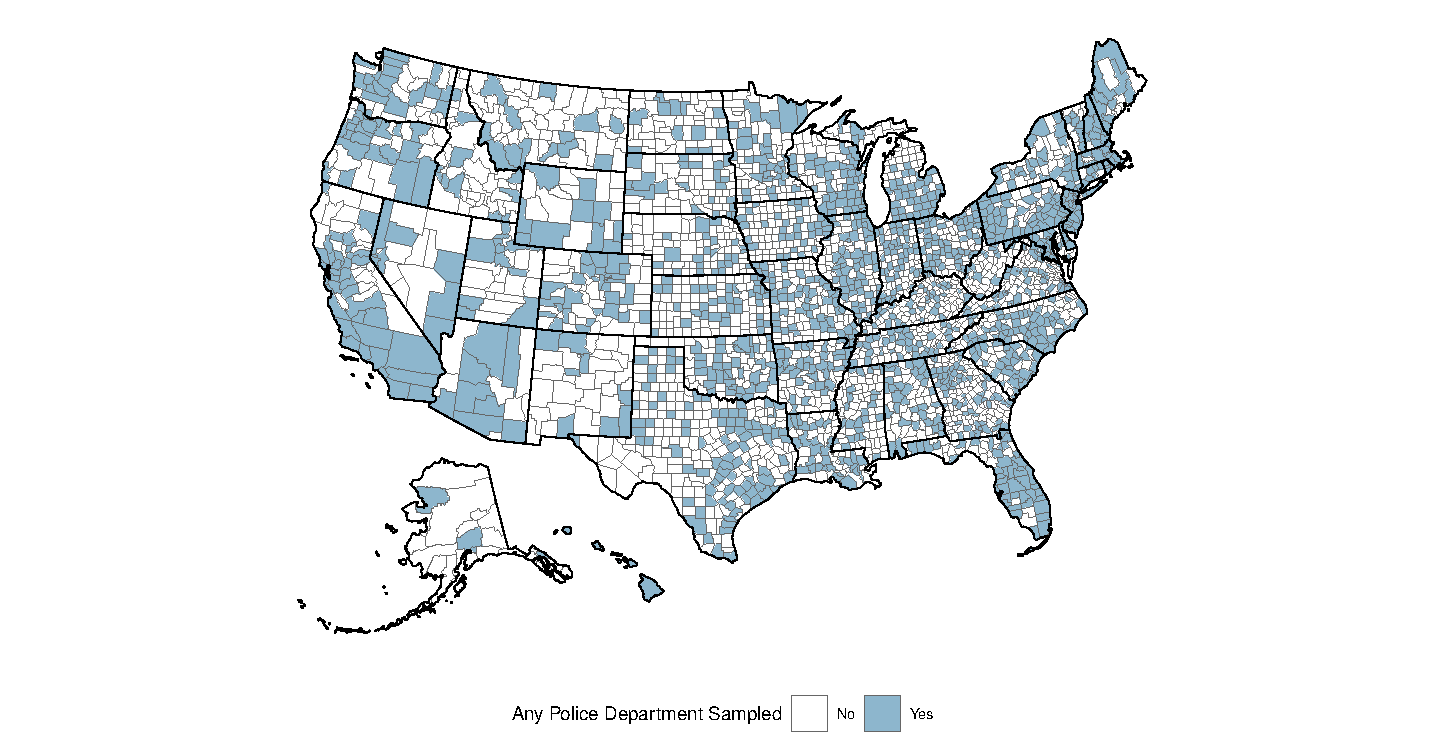
\includegraphics[width = \linewidth]{figures/lemas-map-ct.pdf}
    \label{fig:lemas-geo}
    \fnote{Counties are colored blue where at least one police department within its jurisdiction is surveyed in LEMAS 2016.}
\end{figure}

\begin{figure}[t]  \centering
    \caption{Racial Imagery of Police and White Attitudes toward Policing} 
	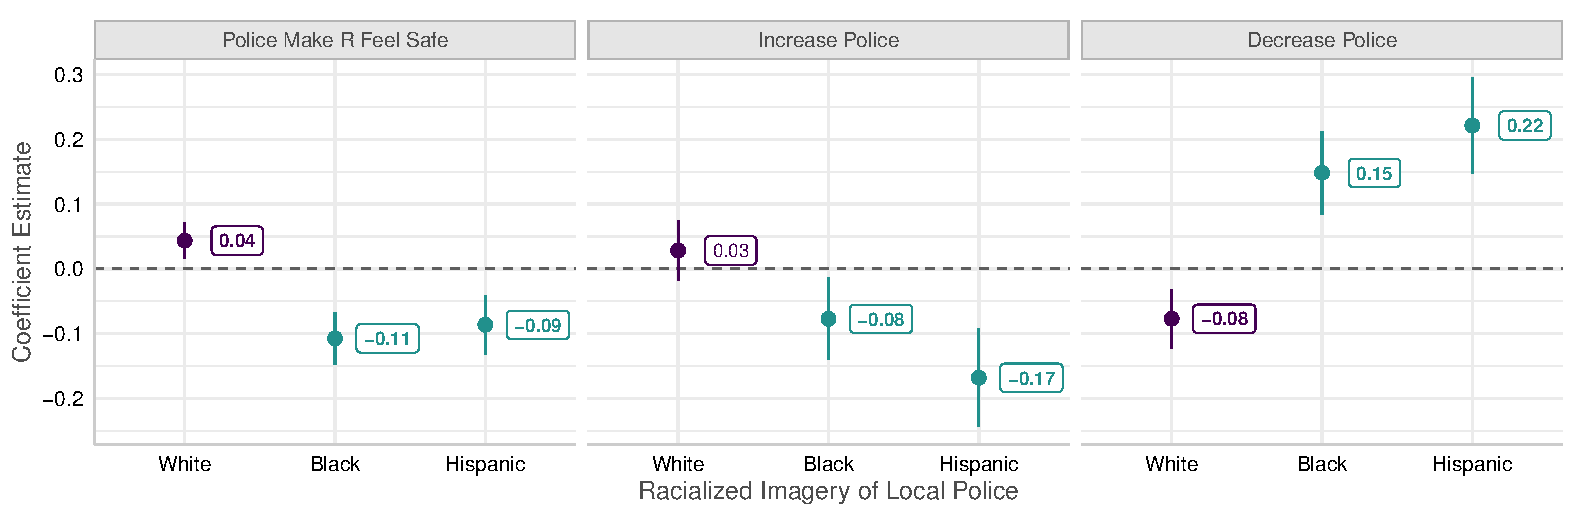
\includegraphics[width = \linewidth]{figures/imagery & attitudes 2}
    \label{fig:baseline}
    \fnote{}
\end{figure}

\begin{figure}[t]  \centering
    \caption{Racial Divides on Policing Moderated by Racial Imagery of Police}
	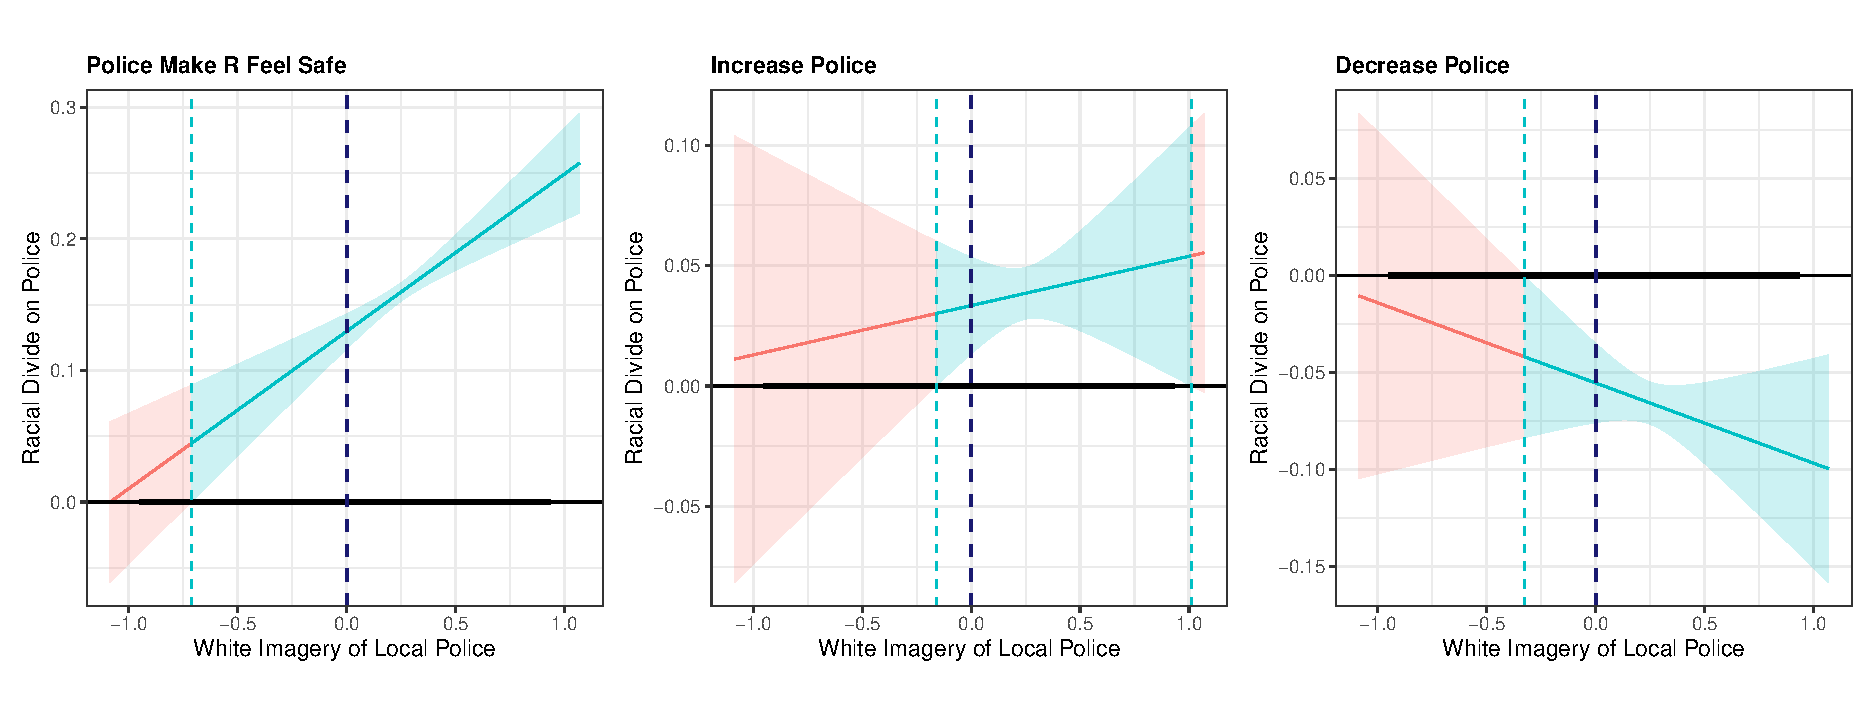
\includegraphics[width = \linewidth]{figures/divide moderation}
    \label{fig:divides}
    \fnote{}
\end{figure}

\begin{figure}[t]  \centering
    \caption{Racial Imagery Moderates Whites' Attitudinal Reaction to Police Violence}
	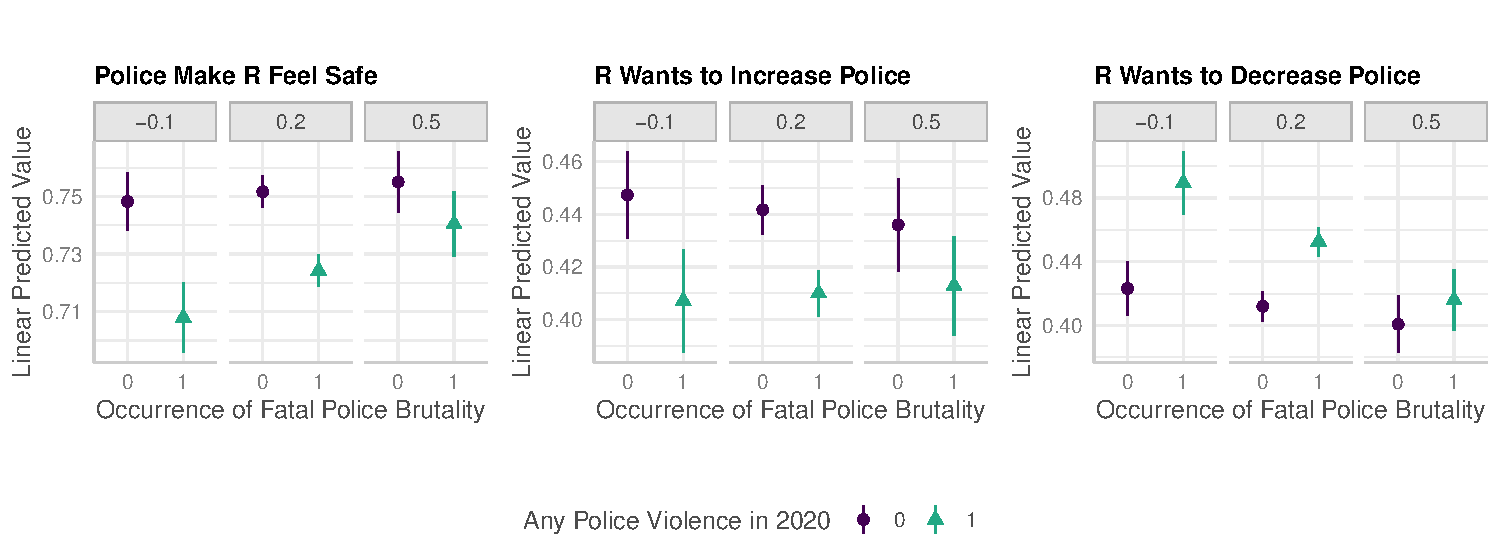
\includegraphics[width = \linewidth]{figures/reaction moderation}
    \label{fig:moderation}
    \fnote{}
\end{figure}

\begin{figure}[t]  \centering
    \caption{Moderation Effect of Racial Imagery Contingent upon Racial Groups Victimized by Police Violence}
	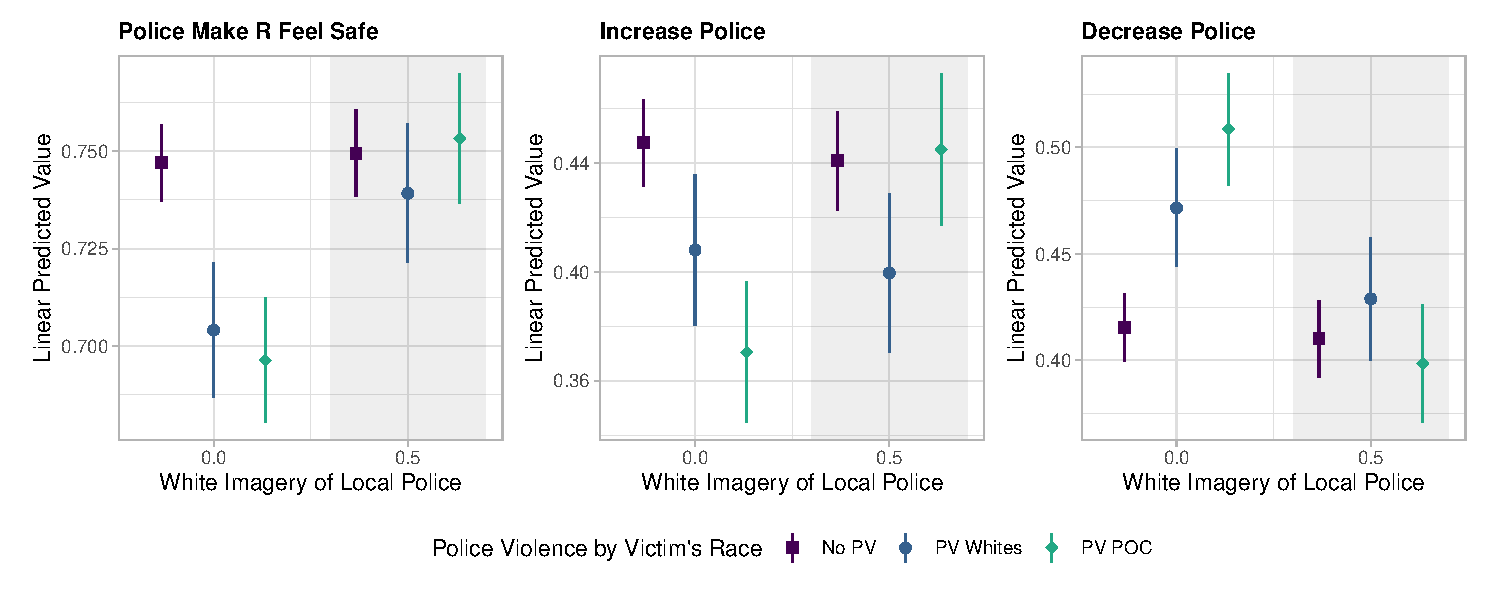
\includegraphics[width = \linewidth]{figures/racial component}
    \label{fig:racial component}
    \fnote{}
\end{figure}


\begin{table}

\caption{Racial Imagery of Local Police Affects Racial Divide on Policing.}
\centering
\begin{tabular}[t]{lccc}
\toprule
  & Police Felt as Safe & Increase Police & Decrease Police\\
\midrule
Racial Divide & 0.221*** & 0.048** & -0.072***\\
 & (0.016) & (0.016) & (0.016)\\
White Imagery of Police & -0.168*** & 0.003 & 0.018\\
 & (0.049) & (0.048) & (0.048)\\
Racial Divide × White Imagery & 0.182** & 0.019 & -0.039\\
 & (0.055) & (0.057) & (0.055)\\
\midrule
Num.Obs. & 39551 & 39597 & 39589\\
R2 & 0.076 & 0.002 & 0.007\\
\bottomrule
\multicolumn{4}{l}{\rule{0pt}{1em}This is the note of your regression table.}\\
\multicolumn{4}{l}{\rule{0pt}{1em}+ p $<$ 0.1, * p $<$ 0.05, ** p $<$ 0.01, *** p $<$ 0.001}\\
\end{tabular}
\end{table}


\begin{table}

\caption{Racial Imagery of Local Police Moderates Attitudinal Reaction to Police Violence.}
\centering
\begin{tabular}[t]{lccc}
\toprule
  & Police Felt as Safe & Increase Police & Decrease Police\\
\midrule
White Imagery of Police & \num{0.006} & \num{-0.009} & \num{-0.014}\\
 & (\num{0.018}) & (\num{0.029}) & (\num{0.029})\\
Any Police Violence in 2020 & \num{-0.047}*** & \num{-0.057}*** & \num{0.074}***\\
 & (\num{0.008}) & (\num{0.013}) & (\num{0.013})\\
Police Violence × White Imagery & \num{0.087}** & \num{0.078}+ & \num{-0.142}**\\
 & (\num{0.028}) & (\num{0.045}) & (\num{0.045})\\
\midrule
Num.Obs. & \num{26016} & \num{26039} & \num{26036}\\
R2 & \num{0.004} & \num{0.002} & \num{0.003}\\
\bottomrule
\multicolumn{4}{l}{\rule{0pt}{1em}This is the note of your regression table.}\\
\multicolumn{4}{l}{\rule{0pt}{1em}+ p $<$ 0.1, * p $<$ 0.05, ** p $<$ 0.01, *** p $<$ 0.001}\\
\end{tabular}
\end{table}


\begin{table}

\caption{Moderating Effect of Racial Imagery Depends upon Racial Groups Victimized by Police Violence}
\centering
\begin{tabular}[t]{lccc}
\toprule
  & Police Felt as Safe & Increase Police & Decrease Police\\
\midrule
White Imagery of Police & 0.007 & -0.013 & -0.010\\
 & (0.027) & (0.029) & (0.029)\\
PV Whites & -0.065*** & -0.039* & 0.056***\\
 & (0.015) & (0.016) & \vphantom{1} (0.016)\\
PV POC & -0.076*** & -0.077*** & 0.093***\\
 & (0.015) & (0.016) & (0.016)\\
White Imagery × PV Whites & 0.098+ & -0.003 & -0.075\\
 & (0.053) & (0.057) & (0.057)\\
White Imagery × PV POC & 0.164** & 0.162** & -0.210***\\
 & (0.053) & (0.058) & (0.058)\\
\midrule
Num.Obs. & 26016 & 26039 & 26036\\
R2 & 0.004 & 0.002 & 0.003\\
\bottomrule
\multicolumn{4}{l}{\rule{0pt}{1em}This is the note of your regression table.}\\
\multicolumn{4}{l}{\rule{0pt}{1em}+ p $<$ 0.1, * p $<$ 0.05, ** p $<$ 0.01, *** p $<$ 0.001}\\
\end{tabular}
\end{table}





\end{appendix}
%===================End Document===================
\end{document}

 